\cite{wei_characterization_2020} -- Characterization of many-body mobility edges with random matrices


\cite{pal_many-body_2010} -- The many-body localization phase transition



\begin{figure}[h]
    \centering
    \addletter{107}{a}
    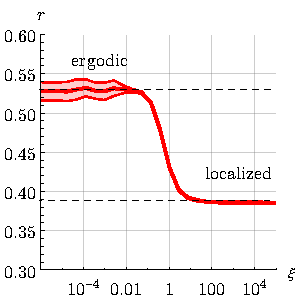
\includegraphics[width=0.225\textwidth]{imgs/erg_reg_add1.pdf}
    \hspace{10 mm} 
    \addletter{107}{b}
    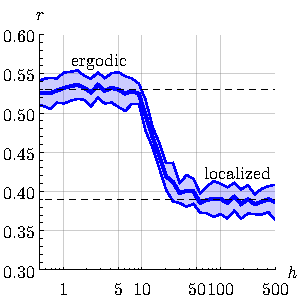
\includegraphics[width=0.225\textwidth]{imgs/erg_reg_add2.pdf}
    \caption{Phase transition with random binary matrix (red) and 1D  spins / fermions (blue)}
    %\label{fig:}
\end{figure}


\begin{figure}[h]
    \centering
    \addletter{50}{a}
    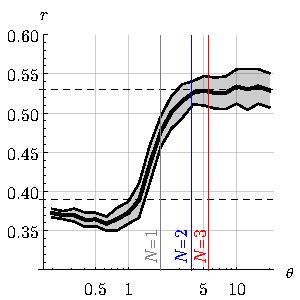
\includegraphics[align=c, width=0.225\textwidth]{imgs/ergodic_reg.pdf}
    \hspace{10 mm} 
    \addletter{50}{b}
    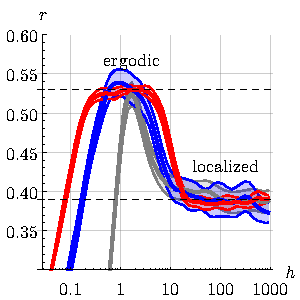
\includegraphics[align=c, width=0.225\textwidth]{imgs/transition.pdf}
    \hspace{5 mm} 
    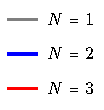
\includegraphics[align=c, width=0.075\textwidth]{imgs/transition_leg.pdf}
    \caption{
    	The influence of matrix rarefaction $\theta$ on phase formation 
    % N=200
    % $\xi=0.01$, $L=20$
    }
    %\label{fig:}
\end{figure}
